\def\mytitle{IDE ASSIGNMENT 1}
\def\mykeywords{}
\def\myauthor{Panjugala Shashikala}
\def\contact{sashipanjugala@gmail.com}
\def\mymodule{}
% #######################################
% #### YOU DON'T NEED TO TOUCH BELOW ####
% #######################################
\documentclass[10pt, a4paper]{article}
\usepackage[a4paper,outer=1.5cm,inner=1.5cm,top=1.75cm,bottom=1.5cm]{geometry}
\twocolumn
\usepackage{graphicx}
\graphicspath{{./images/}}
%colour our links, remove weird boxes
\usepackage[colorlinks,linkcolor={black},citecolor={blue!80!black},urlcolor={blue!80!black}]{hyperref}
%Stop indentation on new paragraphs
\usepackage[parfill]{parskip}
%% Arial-like font
\usepackage{lmodern}
\renewcommand*\familydefault{\sfdefault}
%Napier logo top right
\usepackage{watermark}
%Lorem Ipusm dolor please don't leave any in you final report ;)
\usepackage{circuitikz}
\usetikzlibrary{calc}
\usepackage{tikz}

\usetikzlibrary{shapes, arrows, chains, decorations.markings,intersections,calc}
\usepackage{lipsum}
\usepackage{xcolor}
\usepackage{listings}
%give us the Capital H that we all know and love
\usepackage{float}
%tone down the line spacing after section titles
\usepackage{titlesec}
%Cool maths printing
\usepackage{amsmath}
\usepackage{tabularx}
%PseudoCode
\usepackage{algorithm2e}

\titlespacing{\subsection}{0pt}{\parskip}{-3pt}
\titlespacing{\subsubsection}{0pt}{\parskip}{-\parskip}
\titlespacing{\paragraph}{0pt}{\parskip}{\parskip}
\newcommand{\figuremacro}[5]{
    \begin{figure}[#1]
        \centering
        \includegraphics[width=#5\columnwidth]{#2}
        \caption[#3]{\textbf{#3}#4}
        \label{fig:#2}
    \end{figure}
}

\lstset{
frame=single, 
breaklines=true,
columns=fullflexible
}


\title{\mytitle}
  \author{\myauthor\hspace{1em}\\\contact\\IITH-Future Wireless Communications(FWC22097)\hspace{0.5em}\hspace{0.5em}\mymodule}
\date{}
\hypersetup{pdfauthor=\myauthor,pdftitle=\mytitle,pdfkeywords=\mykeywords}
\sloppy
% #######################################
% ########### START FROM HERE ###########
% #######################################
 
 \begin{document}
 \maketitle
     \tableofcontents 
    \begin{figure}
        \centering
        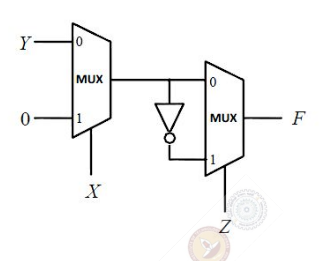
\includegraphics[width=\linewidth]{mux.png}
        \caption{\textbf{The logic realised by the circuit shown in figure is}}
        \label{fig:my_label}
    \end{figure}
  \textbf{}{\mykeywords}
\section{Introduction}
  
    \paragraph{Mutiplexer}
    is a combinational  logic circuit designed to switch one  of  the several  inputs lines through a single common output line by the application of a control signal.
      \\ The implementation of multiplexer takes three steps\\1.To get the truth table of multiplexer\\2.To get the Boolean equation using the truth table by using k map.\\
      \section{Components}
     
       \begin{tabularx}{0.35\textwidth} { 
  | >{\raggedright\arraybackslash}X 
  | >{\centering\arraybackslash}X 
  | >{\raggedleft\arraybackslash}X | }
\hline
\textbf{Component} &  \textbf{Value} & \textbf{Quantity}\\
\hline
Arduino UNO &  & 1 \\  
\hline
Bread board & - & 1 \\
\hline
Jumper wires & M-M & 7 \\
\hline
Resistor & 150 ohm & 1 \\
\hline
Led & - & 1\\
\hline
\end{tabularx}
\begin{center}
    Figure-2 Components
\end{center}
       \subsection{Arduino} \vspace{5mm}
      The Arduino uno has some ground pins, analog input pins A0-A5 and digital pins D1-D13 that can be used for both input as well as output. It also has two power pins that can generate 3.3V and 5V.In the following exercises, only the ground, 5V and digital pins will be used.
    \section{Truth Table of 2x1 Multiplexer}
    \begin{figure}
        \centering
        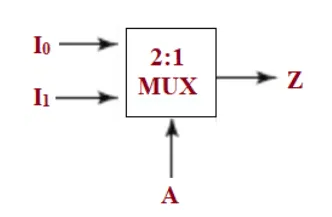
\includegraphics[width=\linewidth]{2x1_mux.png}
        \caption{\textbf{2x1 Multiplexer}}
        \label{fig:my_label}
    \end{figure}  
    
        The truth table for 2x1 Multiplexer as follows: \\Selection line=A and output is Z
  
 \begin{tabularx}{0.35\textwidth} { 
  | >{\raggedright\arraybackslash}X 
  | >{\centering\arraybackslash}X 
  | >{\raggedleft\arraybackslash}X | }
\hline
A & Z \\
\hline
0 & I0 \\  
\hline
1 & I1 \\ 
\hline

\end{tabularx}
             \\By using the above truth table and from figure 2. we get the boolean equation as:\\F=A'I0+AI1.
             
	


       
  \section{Boolean Equation}
  
  
 By solving the given multipexer circuit diagram we get the boolean equation as follows:\\F=X'YZ'+XY+Y'Z
 %Using the above Boolean Equation the circuit diagram is drawn as:
  %  \begin{center}

%\begin{circuitikz} \draw
%(0,3) node[xor port, number inputs=3] (xor) {};
%\node[left] at (xor.in 1) {\(C\)};
%\node[left] at (xor.in 2) {\(A\)};

%\node[left] at (xor.in 3) {\(B\)};
%\node[right] at (xor.out) {\(F(Output)\)};
%\node[right] at (and.out) {\(F=(X+Y)(X+Z')(X'+Y'+Z)\)};
%\end{circuitikz}

%    \end{center}

%\begin{center}
 
 
 %    Figure-4 xor operation
%\end{center}
\section{Truth table of given multiplexer circuit}
		The truth table of given multiplexer circuit diagram is as:
 \begin{tabularx}{0.35\textwidth} {
  | >{\raggedright\arraybackslash}X 
  | >{\centering\arraybackslash}X 
  | >{\centering\arraybackslash}X 
  | >{\raggedleft\arraybackslash}X | }
\hline
X & Y & Z & F \\
\hline
0 & 0 & 0 & 0 \\
\hline
0 & 0 & 1 & 1 \\
\hline
0 & 1 & 0 & 1 \\
\hline
0 & 1 & 1 & 0 \\
\hline
1 & 0 & 0 & 0 \\
\hline
1 & 0 & 1 & 1 \\
\hline
1 & 1 & 0 & 1 \\
\hline
1 & 1 & 1 & 1 \\
\hline
\end{tabularx}

\section{Hardware}
1. Connect Arduino to the computer and upload the code in to the arduino.Make 2,3,4 pins as input pins and 13 pin as output pin. Corresponds to the given inputs for the selection lines of multiplexer the outputs will be obtained at 13 pin. The led will glow when the output of the given boolean function is high.

vspace{10mm}    

\section{Software}
 Download the following code
 \begin{lstlisting}
https://github.com/PanjugalaShashikala/FWC_2022097/blob/main/ide/main.cpp
 \end{lstlisting}
\end{document}
